\documentclass[12pt, a4paper, titlepage, oneside]{article}

% On commence par enjoliver
\usepackage[francais]{babel}	%typographie française
\usepackage[utf8]{inputenc}	% accents 8 bits dans le source
\usepackage[T1]{fontenc}	% accents dans le DVI
\usepackage{lmodern}	% Sans cette ligne la typo va être merdique!!!
\usepackage[usenames,dvipsnames]{color}
%\usepackage{nicebox}
% on inclue de l'utilitaire
\usepackage{float}
\usepackage{graphicx}
\usepackage{listings}
\newcommand{\Hrule}{\rule{\linewidth}{0.5mm}}

%On va se faire de belles marges
\usepackage{vmargin}
\setmarginsrb{1.5cm}{1.5cm}{1.5cm}{1.5cm}{15.71402pt}{1.5cm}{0.5cm}{1.5cm}

% de jolis headers/footers
\usepackage{fancyhdr}
\pagestyle{fancy}
\renewcommand{\sectionmark}[1]{\markright{\thesection\ #1}}
\renewcommand{\headrulewidth}{0.5pt}
\renewcommand{\footrulewidth}{0.5pt}
\fancyhead{} % clear all header fields
\fancyhead[L]{Implémentation de l'algorythme de Ricart et Agrawala}
\fancyhead[R]{\rightmark}
\fancyfoot{} % clear all footer fields
\fancyfoot[C]{\thepage}

%Gui : problème du absence conférence
%Gui : 

\begin{document}
	% on commence par la page de garde
	%\begin{changemargin}
\begin{titlepage}
	\begin{minipage}{0.5\textwidth}
		\begin{flushleft} \large
			%
\includegraphics[bb=0 0 110 30]{images/logo-isima.png}\\
			
\includegraphics[width=3.8cm]{./schema/logo-isima.jpg}\\
		\end{flushleft}
	\end{minipage}
	\begin{minipage}{0.43\textwidth}
		\begin{flushright} \large
			
\includegraphics[width=3.8cm]{schema/logo-boost.png}
		\end{flushright}
	\end{minipage}

	\begin{minipage}{0.5\textwidth}
		\begin{flushleft} \large
			\textbf{I}nstitut \textbf{S}upérieur\\
			d'\textbf{I}nformatique de\\
			\textbf{M}odélisation et de\\
			leurs \textbf{A}pplications\\
			~\\
% 			\begin{small}
% 			Complexe des Cézeaux \\
% 			BP 125\\
% 			63173 Aubière Cedex
% 			\end{small}
		\end{flushleft}
	\end{minipage}
	\begin{minipage}{0.43\textwidth}
		\begin{flushright} \large
		\end{flushright}
	\end{minipage}


		\vfill
		\begin{center}
			\Hrule \\[0.4cm]
			\Large{Rapport de Projet de troisième année}\\		
			\Large Filière 5 : Infrastructure entreprise, réseaux et télécoms\\[1.0cm]
			\Huge{Représentation et analyse de la topologie internet}\\
			\Hrule\\[0.8cm]
\vfill 
% \textcolor{red}{\Huge{\textbf{MERCI JULIEN !}}}
% \vfill 
		\end{center}
		
		\vfill
		\begin{minipage}{0.5\textwidth}
			\begin{flushleft} \large
				\emph{Auteurs:}\\
				 Bastien \textsc{Legrand}\\
				 Jan \textsc{Villeminot}

			\end{flushleft}
		\end{minipage}
		\begin{minipage}{0.45\textwidth}
			\begin{flushright} \large
				\emph{Tuteur de projet:} \\
				Mickael \textsc{Meulle}\\
			\end{flushright}
		\end{minipage}
		
		\vfil
		\begin{center}
			{\large 2008-2009}
		\end{center}
	\end{titlepage}
%\end{changemargin}
	%\par
Internet, le réseau des réseaux, est une interconnexion de systèmes autonomes, réseaux indépendents et raccordés entre eux. Compte tenu de sa taille, représenter Internet est une entreprise des plus difficiles.

Le projet avait pour but de réaliser un outil permettant d'afficher et d'analyser la topologie de l'Internet. La finalité est de proposer un programme évolutif qui facilite l'implémentation de nouvelles méthodes d'affichage et d'analyse. Ses objectifs en cachent un plus pédagogique : maîtriser les outils à notre disposition et les utiliser lors du développement du logiciel.

Articulé autour du patron Modèle Vue Contrôleur, le logiciel est basé sur la librairie graphe de \boost qui réalise tous les traitements de construction et de manipulation sur la topologie. L'interface graphique, réalisée en Qt est totalement indépendante de la partie traitement et permettra donc l'ajout de fonctionnalités facilement.

En cons\'equence, le travail de d\'eveloppement est parallelisable : une personne travaillant plus sur l'interface graphique, l'autre sur la couche de coeur. L'association des diff\'erentes parties est facilit\'ee par l'utilisation d'un gestionnaire de source : git.

L'affichage de la topologie a un rendu circulaire et est accompagné d'une fonction de zoom et d'un certain nombre de fonctions de filtrage et de calcul pour permettre à l'utilisateur, selon ses besoins, de se focaliser sur un aspect précis du graphe.

Finalement, l'outil r\'ealis\'e est \'evolutif, performant et son d\'eveloppement nous a permis d'approfondir nos connaissances dans les outils utilis\'es.\\

mots cl\'e : boost, Qt, interface graphique, évolutivité, topologie de l'Internet, git








	%\section*{Remerciements}

Nous tenons \`a remercier tout particuli\`erement Monsieur Mickael Meulle, notre tuteur de projet, pour son accompagnement tout au long du parcours et pour sa disponibilit\'e malgr\'e la distance.	
	% puis vient la table des matières
	%\pagenumbering{roman}
%	\listoffigures
%\pagebreak
 %	\tableofcontents
%	\pagebreak\textit{\textit{}}
%\fancyhead[R]{Lexique}
	%\input{Lexique.tex}
 %	\pagebreak
        
	%\fancyhead[R]{Introduction}
	%\section*{Introduction}

\subsection*{Le contexte}
\frame
{
\frametitle{Pr\'esentation du contexte}


}

\subsection*{Les objectifs}
\frame
{
\frametitle{Pr\'esentation des objectifs}


}
	\pagebreak 	
% 	% puis la page d'intro
\fancyhead[L]{Systemes Repartis}
\fancyhead[R]{\rightmark}
	
% 	\fancyhead{}
% 	\fancyhead[R]{Rapport de Design Électronique}
% 	\section*{Introduction}

\subsection*{Le contexte}
\frame
{
\frametitle{Pr\'esentation du contexte}


}

\subsection*{Les objectifs}
\frame
{
\frametitle{Pr\'esentation des objectifs}


}
% 	\pagebreak
	\section{Les donn\'ees, les outils}

\begin{frame}
 	\frametitle{Les donn\'ees, les outils}
        \tableofcontents[currentsection,hideothersubsections]
\end{frame}

\subsection{Les donn\'ees}
\frame
{
\frametitle{Les donn\'ees}
3 sources : \\
\begin{itemize}
 \item traceroute
 \item WHOIS
 \item BGP
\end{itemize}
~\\
Source retenue : BGP = la plus fiable
}

\subsection{Outils d'analyse}
\frame
{
\frametitle{Outils d'analyse}
Outils fournis par la RO et la Th\'eorie des graphes : \\
\begin{itemize}
 \item Structure de graphe connexe,
 \item Zone de forte densit\'e de liens : full-mesh / clique,
 \item Liens les plus importants : centralit\'e.
\end{itemize}
}

\subsection{Outils de d\'eveloppement}
\frame
{
\frametitle{Outils de d\'eveloppement}
% \begin{block}{La librairie Boost}
%  Ensemble de biblioth\`eques logicielles C++\\
%  Utilisation du module \textit{Graph}\\
%  \begin{center}
%   
\includegraphics[width=4cm]{logo-boost}
%  \end{center}
% \end{block}
% 
% \begin{block}{Qt}
%  Biblioth\`eque logicielle orient\'ee objet en C++\\
%  Composants graphiques pour l'IHM\\
%  \begin{center}
%   
\includegraphics[width=4cm]{logo-qt}
%  \end{center}
% \end{block}

\begin{minipage}{0.45\textwidth}
\begin{flushleft}
\begin{block}{La librairie Boost}
\begin{itemize}
\item Ensemble de biblioth\`eques C++
\item Utilisation du module \textit{graph}
 \end{itemize}
\end{block}
\end{flushleft}
\end{minipage}
\hfill
\begin{minipage}{0.45\textwidth}
\begin{flushright}
\begin{center}

\includegraphics[width=4cm]{logo-boost.png}
\end{center}
\end{flushright}
\end{minipage}
\vfill
\begin{minipage}{0.45\textwidth}
\begin{flushleft}
\begin{center}

\includegraphics[width=2cm]{logo-qt.png}
\end{center}
\end{flushleft}
\end{minipage}
\hfill
\begin{minipage}{0.45\textwidth}
\begin{flushright}
\begin{block}{La librairie Qt}
\begin{itemize}
\item Biblioth\`eque logicielle orient\'ee objet en C++
\item Composants graphiques pour l'IHM
\end{itemize}
\end{block}
\end{flushright}
\end{minipage}
}
\pagebreak
\section{Le logiciel de visualisation et d'analyse de l'internet}
\subsection{Objectifs}
Le but du projet est de produire un logiciel qui permette la visualisation de la topologie d'internet :
\subsubsection{Objectifs de l'application}
\label{obj}
\paragraph{Analyse de la topologie}
Construire un graphe contenant la topologie d'internet et permettant son analyse en se servant des méthodes disponibles dans la librairie graphe de \textit{Boost}.

\paragraph{Affichage de la topologie}
Réaliser une interface agréable dans la librairie de notre choix et lui permettre d'afficher l'intégralité de l'analyse réalisée.

\subsubsection{Objectif pédagogiques}
Au delà, de l'objectif de réalisation d'une application et de l'organisation que cela suppose. Un certains nombre d'objectifs pédagogique ont été fixés par notre tuteur ou par nous-même.

\paragraph{Objectifs fixés dès le départ : } 
\paragraph{}L'objectif principal est bien évidemment d'apprendre à maîtriser la librairie boost de C++, principalement sa partie sur les graphs. Il était aussi question d'approfondir notre connaissance de la topologie d'internet.

\paragraph{Objectifs personnels suppl\'ementaires : }
\paragraph{} En outre, nous nous sommes nous-même fixés des objectifs. En effet, l'utilisation d'une librairie graphique pour représenter la topologie d'internet était nécessaire mais son choix nous était réservé. Nous avons choisi d'utiliser Qt, et ce pour deux raisons. La première est que nous voulions approfondir le cours sur Qt que nous allions avoir dans le cadre de nos études à l'ISIMA.

La seconde est que, sous la pression de Nokia, cette librairie est récemment passé sous licence LGPL ce qui veut dire que les développeurs d'applications commerciales vont pouvoir développer gratuitement autour de Qt (sans payer les très onéreuses licences jusqu'à présent nécessaires pour vendre quelque chose). Il est fort probable que Qt prennent beaucoup plus d'ampleur dans les prochaines années.

\paragraph{} Nous nous sommes fixés un autre objectif, celui d'apprendre à utiliser git, pour les raisons évoqué en \ref{gitPar} subversion ne nous convenait pas, mais nous ne connaissions pas vraiment git pour autant, néanmoins après avoir visionner une conférence de Linus Torvalds sur le sujet, il nous a semblé logique et nécessaire d'appréhender git et de s'en servir pour le projet. D'autant plus que l'un comme l'autre nous avions effectué nos stages avec subversion ou cvs.

\subsubsection{Déroulement du projet}

Nous n'avons que très peu vu notre tuteur de projet en personne, la quasi totalité du projet a été mené par des échanges de mails, et des discussions sur des messageries instantannées (Skype, gchat). De plus, il nous a donné une grande autonomie sur les décisions à prendre pour mener à bien nos objectifs.

En contre-partie, cela demande une bonne organisation. En effet, quelques soient les décisions ou les problèmes rencontrés, il faut en rendre compte au tuteur lors de la prochaine réunion de travail suivante, réunion qui avait régulièrement lieu le Jeudi après-midi.

\subsubsection{Méthode de travail}

Afin d'optimiser la production, nous avons adopté une méthode de développement par itération. En fait, nous nous sommes répartis les tâches selon des fonctionnalités ``élémentaires'', par exemple afficher le graph avec Circle Graph Layout ou réaliser l'extension du file\_parser permettant de trouver les AS de transit. Après avoir isolé l'ensemble des fonctionnalités nécessaires d'une semaine à l'autre, nous affectons des priorités aux une est aux autres afin de pouvoir mieux répartir les tâches entre les différents membres du binôme.

\subsubsection{La librairie graph de boost}
%\documentclass[a4paper,12pt]{article}

%\begin{document}

% \subsection{La librairie \boost}

\subparagraph{}
La librairie \boost  est un ensemble de biblioth\`eques logicielles C++ dont le but est de compléter et de parfaire les fonctionnalités du langage et la librairie stl. La librairie \boost est compos\'ee de nombreux modules parmis lesquels on retrouve des fonctionnalit\'es de bases comme les entr\'ees / sorties ou la gestion des erreurs, mais aussi d'autres plus avanc\'ees comme des fonctions de gestion de graphes, de programmation lin\'eaire, de g\'en\'eration de nombres pseudo-al\'eatoires, de traitement d'images ou de multithreading.
\par
L'\'ecriture de nouveaux \'el\'ements pour la librairie \boost est soumise \`a un  comit\'e de lecture et l'ensemble des biblioth\`eques est plac\'e sous une licence sp\'eciale : la \textit{Boost Software Licence} qui permet d'inclure des modules \boost aussi bien dans des projets Open Source que dans des projets propri\'etaires.
\par
\'Etant donn\'e que nombre des membres du comit\'e de lecture font aussi partie du comit\'e du standard C++, plusieurs biblioth\`eques issues de la \boost ont \'et\'e s\'electionn\'ees pour faire partie de la prochaine norme du C++.
\par
Au cours de notre projet nous avons beaucoup utilis\'e la partie gestion de graphes de \boost ainsi que certaines des fonctions d'entr\'es / sorties am\'elior\'ees.
%\end{document}



\subsubsection{La librairie graphique Qt}
\subparagraph{}
Qt, prononcer ``cute'' de l'anglais joli, est une biblioth\`eque logicielle orient\'ee objet et d\'evelopp\'ee en C++ par la soci\'et\'e \textit{Qt Software}, anciennement connue sous le nom de \textit{Trolltech}. Elle offre des composants graphique permettant entre autre l'acc\`es aux donn\'ees, les connexions r\'eseaux, la gestion des files d'ex\'ecution. Cette biblioth\`eque est aujourd'hui dans sa version quatre.
\subparagraph{}
Qt permet la portabilit\'e des applications par simple recompilation du code source. Elle est support\'ee sous des environnements tels que Unix/Linux, Windows et Mac OS X.
\subparagraph{}
Qt est principalement connue pour \^etre la biblioth\`eque sur laquelle repose l'environnement graphique KDE, l'un des environnements de bureau le plus utilis\'e dans le monde Linux. En outre, un certain nombre d'applications tr\`es connues du grand public utilisent Qt : VLC Media Player, Skype, Google Earth...

\par
L'outil Qt repose sur trois parties essentielles : 
\begin{itemize}
	\item Les slots et les signaux,
	\item Qt Designer,
	\item Le compilateur de meta-objet MOC.
\end{itemize}

\subparagraph{}
Qt Designer est un outil graphique permettant de créer facilement des interfaces graphiques avec Qt, d'y ajouter des panneaux, des boutons et d'y connecter des fonctions sous la forme de signaux et de slots. Au cours de notre projet, nous n'avons que tr\`es peu utilis\'e cet outil, pr\'ef\'erant explorer les \'etapes de cr\'eation d'une interface graphique en r\'ealisant nous m\^eme tout le code.
\subparagraph{}
Les slots et signaux sont les m\'ecanismes sp\'ecifiques \`a Qt qui lui permettent de g\'erer les \'echanges d'informations entre les diff\'erents \'el\'ements d'une interface graphique. Il s'agit en fait d'une impl\'ementation un peu particulière du patron de conception observateur.
Les objets Qt poss\`edent des slots et des signaux. Un objet peut \'emettre des signaux qui seront re\c cus par les slots d'un autre objet. Ainsi, si on veut cr\'eer un bouton ``quitter'' dans une fen\^etre, il faut connecter le signal correspondant à l'action \textit{je clique sur le bouton} au slot \textit{la fen\^etre se ferme}.
\subparagraph{}
Le compilateur de m\'eta-objets MOC (Meta Object Compiler) est un pr\'eprocesseur qui est appliqu\'e au code source de l'application avant sa compilation et qui r\'eunit les informations n\'ecessaires au fonctionnement des slots et signaux, voir \'eventuellement \`a l'introspection. \subparagraph{}
L'introspection est la capacit\'e qu'a un programme à connaître son \'etat, examiner ses structures internes et \'eventuellement modifier des objets le composant au cours de l'\'execution. Cela va de pair avec les slots et les signaux, puisque pour cacher une fen\^etre, on peut ainsi changer son \'etat de visible \`a non visible.
Un exemple d'introspection est le démon dcop de KDE qui permet de connaitre exactement l'état de chaque composant d'une application KDE, et d'agir dessus. Il est par exemple possible d'arrêter la musique avec Amarok, ou de graver un CD uniquement par introspection avec K3B.
Non présente nativement en C++, la faisabilité de l'introspection est un atout majeur de Qt.

\subsection{Méthodologie de développement et redistribution}
\subsubsection{Documentation avec Doxygen}
\par
Doxygen est un outil permettant la génération de documentation à propos de code, il est utilisable avec la plupart des langages de programmation actuels (C/C++, Java, python, Groovy). Son nom est la contraction de \textit{dox} (pour docs, de l'anglais documents) et \textit{gen} (de l'anglais generator). Il a été en grande partie \'ecrit par Dimitri van Heesch. La documentation g\'en\'er\'ee peut \^etre soit en HTML, soit en \LaTeX.

\par Il s'appuie pour cela sur un certains nombre de commentaires \'ecrits dans le code avec une syntaxe sp\'ecifique (voir figure \ref{exemple_doxygen}). Il se base aussi sur une analyse du code qui lui permet d'extraire les prototypes des fonctions, des classes, les fichiers inclus et la documentation relative à ceux-ci.

\par Il peut ensuite repr\'esenter leur hi\'erarchie sous forme de sch\'emas UML. Il crée ensuite une documentation homogène permettant de naviguer à partir d'un index vers les différentes pages de documentation créées.

	La figure 3 nous montre comment définir une br\`eve description du r\^ole de la méthodes, des informations sur ses diff\'erents param\`etres et sur ce qu'elle retourne.

\begin{figure}[H]
        \begin{center}
                \begin{tabular}{l}
                        \hline
                        \verb|\brief Ajoute une arete|\\
                        \verb|\param i1 index du premier point|\\
                        \verb|\param i2 index du deuxieme point} |\\
                        \verb|\param linkType descripteur du type d'arete|\\
			\verb|\param found booleen resultat |\\
			\verb|\param e edge_descriptor de l'arete|\\
			\verb|\param g reference sur le Graph ou il faut ajouter la relation|\\
			\verb|\return le type de point|\\
                        \hline
                \end{tabular}
        \end{center}
\caption{\label{exemple_doxygen} Exemple de syntaxe Doxygen}
\end{figure}


\subsubsection{Redistribution et travail en équipe}
\paragraph{subversion : des limites}
%TODO supprimer premier paragraphe
%EvOr se défoule
%La plupart des personnes ayant utilisé subversion de manière professionnelle en sont conscientes il est loin d'être agréable à utiliser, sa gestion des branches est désastreuses, et les conflits sont gérés de manière abruptes et souvent inefficaces, pour palier à ses défauts les entreprises mettent en place des politiques de fonctionnement autour du gestionnaire de version drastique avec par exemple interdiction de commiter ce qui ne marche pas. Au delà de ses problèmes de fonctionnement subversion est lent, très lent et nécessite en plus la présenced'un serveur pour pouvoir commiter.
%Fin EvOr se défoule

\paragraph{} L'une des bases du développement est d'utiliser un gestionnaire de sources afin de pouvoir modifier ses fichiers sans se soucier des conséquences. La première chose que nous avons faite, avant même de passer au développement, est de mettre en place un serveur subversion sur l'une de nos machines. Le problème qui s'est très vite posé est le suivant : quelque soit l'endroit où l'autre travaille, s'il n'a pas accès au serveur, il ne peut pas l'utiliser (\verb|commit/checkout|) et doit donc développer sans gestionnaire de sources (figure \ref{svn})... Il nous fallait un moyen de contrôler nos sources de manière distribuée : git.

\begin{figure}[H]
\begin{center}
        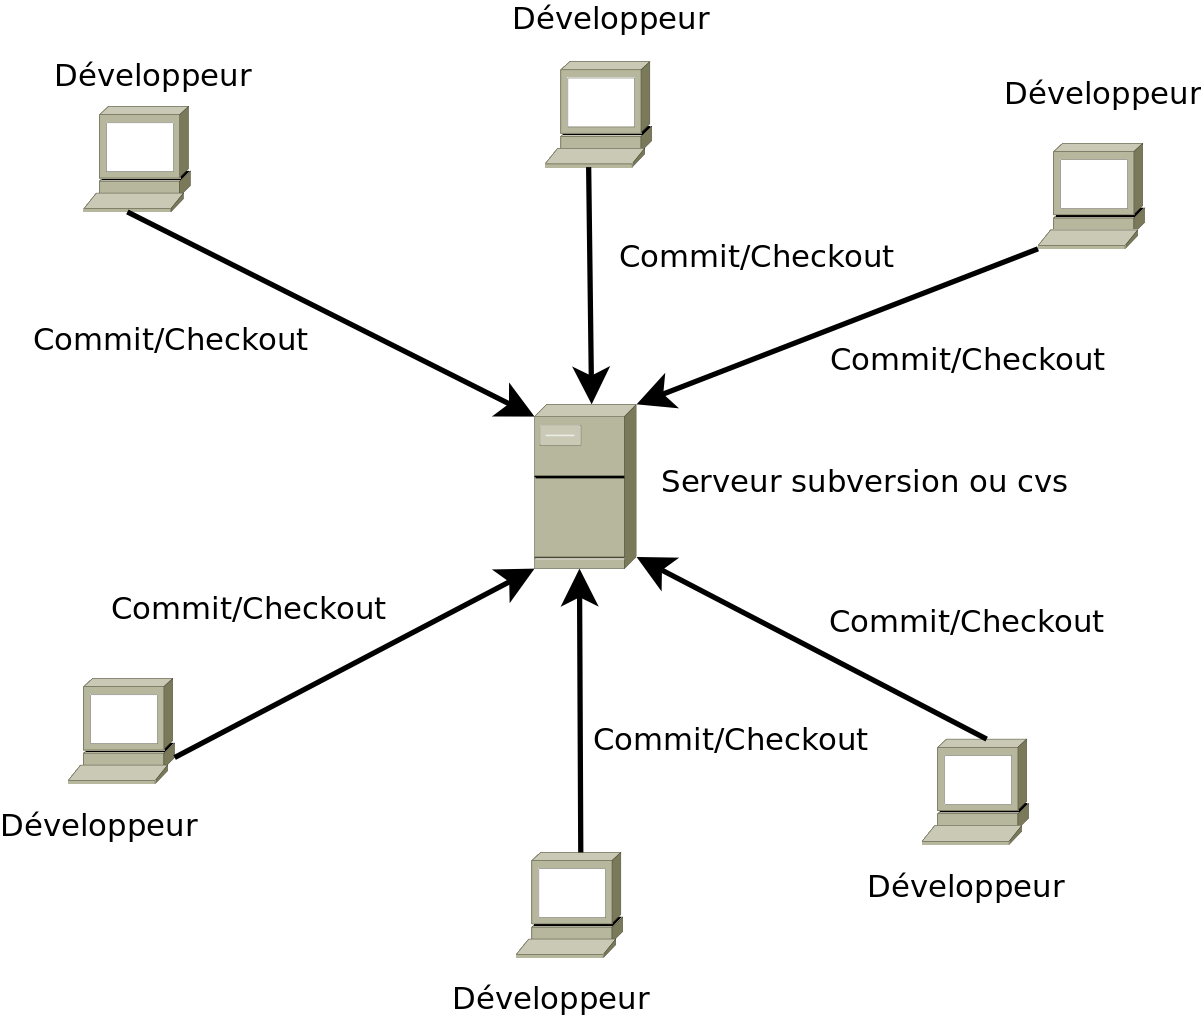
\includegraphics[width=0.7\textwidth]{./schema/svn.png}
\caption{La gestion classique des sources : centralisation totale }
\label{svn}
\end{center}
\end{figure}


\paragraph{git : Le gestionnaire de source distribué}
\label{gitPar}
\paragraph{Histoire :}
\subparagraph{} Git a été créé par Linus Torvalds en 2004, il avait besoin de remplacer BitKeeper pour la gestion des sources du noyau Linux, et il est évident qu'il ne peut pas mettre en place un serveur subversion pour un projet aussi vaste et avec autant de développeurs répartis au quatre coins du monde. Il a donc écrit, en quelques jours, un gestionnaire de sources distribué performant et qui a pour objectif de ne pas géner le développeur. En outre, Git effectue un checksum SHA1 des sources à chaque fois qu'une modifications est effectuée (commit ou push) ce qui permet d'être sûr de l'unicité des données...

\paragraph{Que veut dire distribué ?} 
\subparagraph{}Git est distribué, cela veut dire que chaque machine l'utilisant est un serveur et un client. En d'autres termes, chaque développeur peut ``commiter'' et effectuer des \verb|revert| en local. Ce qui permet de développer de manière beaucoup plus efficace, puisque les commits sont effectués en quelques millisecondes (le temps d'afficher la trace). Une fois que le développeur est satisfait de son travail, il peut demander aux autres de \verb|pull| (récupérer les sources) depuis sa machine, ou il peut \verb|push| (envoyer les sources) sur un serveur de fichiers central par exemple (figure \ref{git}). Tout ce que nécessite git pour fonctionner est un client et/ou un serveur ssh.


\begin{figure}[H]
\begin{center}
        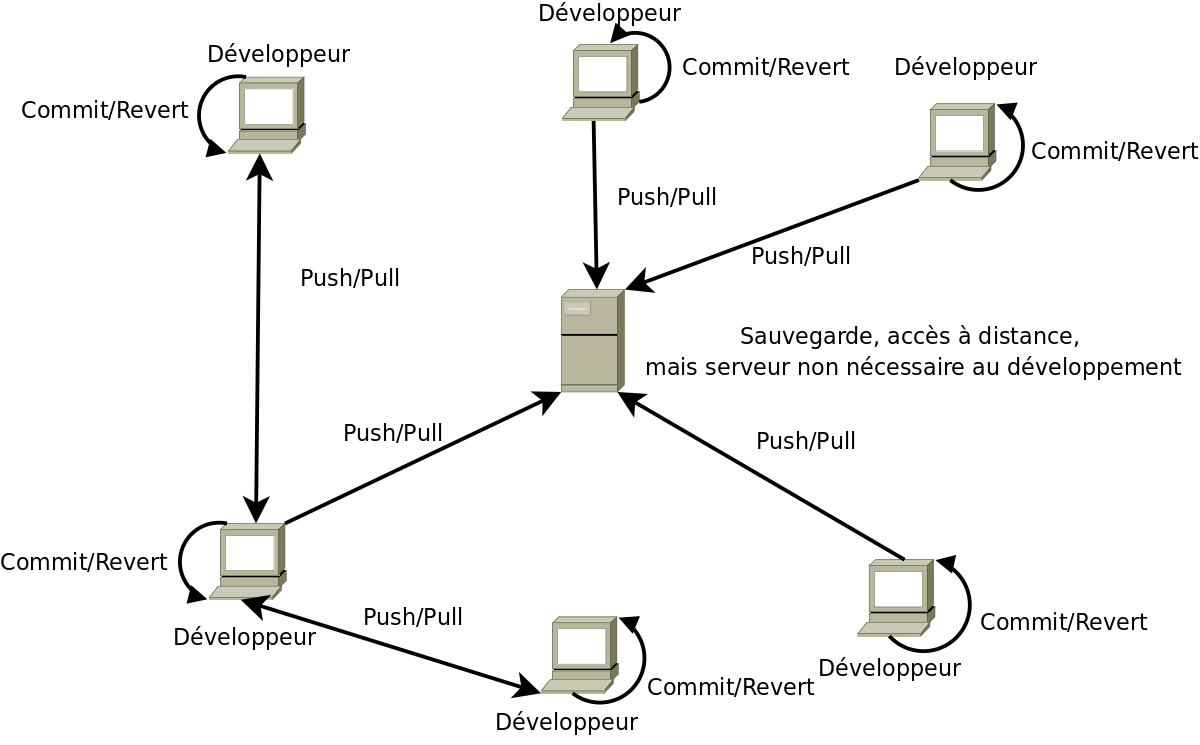
\includegraphics[width=0.8\textwidth]{./schema/git.png}
\caption{La gestion des sources avec git : Distribution et liberté}
\label{git}
\end{center}
\end{figure}

\paragraph{Fonctionnement :} 

\subparagraph{}La comparaison de fichiers sous git est un peu particulière, contrairement à subversion qui se base sur le nom du fichier et le numéro du commit, git se base sur un checksum du fichier. Il se sert en fait d'une base interne contenant l'intégralité des checksums des fichiers en fonction du numéro du commit correspondant mais ne se base que sur le checksum pour vérifier si deux fichiers sont différents, l'opération est donc très rapide et sûr.

\subparagraph{} Concrètement, la clé du fonctionnement de git est l'utilisation massive des branches. En effet, dans git tout est une branche : chaque machine de chaque développeur est une branche et ce de manière totalement transparente. C'est à dire que le développeur peut \verb|commit| et \verb|revert| sa propre branche et l'envoyer ensuite sur la branche principale \verb|push| (\verb|master|). Avec les sources, l'historique des commits effectués en local est envoyé et n'importe quel développeur peut annuler n'importe quel commit...

\subparagraph{} Il est donc très facile de créer, de merger et de supprimer une branche avec git, tellement facile qu'on se demande comment ça peut être aussi difficile avec subversion.

\subparagraph{} En cas de conflit, git ne fait rien ; pour git le simple fait que deux fichiers devant être ``mergés'' soient plus ``récents'' que leur dernière version commune est un conflit. Il signale alors à l'utilisateur qu'il faut ``merger''. Et ce merge est très aisé, il se déroule automatiquement la plupart du temps, à la main parfois : git est capable de ne montrer uniquement les parties de fichiers en conflit.


\subparagraph{}Nous vous renvoyons à notre annexe sur git pour un descriptif détaillé des commandes à connaître avec git.

%TODO en annexe les commandes de git
%Git fonctionne en ligne de commande, néanmoins ses développeur l'ont doté d'une interface graphique plutôt fonctionnelle. Git possède un nombre impressionant de fonctionnalités, nous allons toutefois lister celles qui nous semblemt les plus importantes.

\paragraph{Et l'accès aux données depuis l'extérieur ?}
\subparagraph{} A l'instar de sourceforge pour subversion, il existe quelques sites communautaires permettant de déposer les sources de ses projets sur des serveurs distants, github en fait partie. En choisissant git, nous voulions, outre la puissance et la distribution, avoir accès aux modifications de l'un et de l'autre sans avoir besoin de s'appeler pour se demander d'allumer nos machines.

Centraliser nos sources sur la toile, nous a semblé être la meilleure solution. Github fonctionne avec git, il lui suffit d'avoir votre clé publique rsa et il est possible d'utiliser git avec le site. 

\paragraph{En résumé}

\subparagraph{}L'utilisation conjuguée de git et de github nous permet :
\begin{itemize}
 \item De développer avec un gestionnaire de source sans accès au réseau ;
 \item D'avoir accès à notre projet par une simple commande quelque soit la machine sur laquelle nous travaillons ;
\item De développer avec un outil puissant, rapide et efficace.
\end{itemize}

\subsection{Aperçu du logiciel}



\subsubsection{Modèle Vue Controlleur}
\label{mvcText}
Lorsque l'on développe une application disposant d'une interface graphique, la base du développement est de séparer la partie traitement ou métier de l'interface à proprement parler. Il est souvent utile de rajouter une couche d'interfaçage entre la partie métier et la partie affichage. Cette modélisation s'appelle Modèle Vue Controlleur. Nous avons choisi d'implémenter ce modèle dans notre projet. La partie métier étant le graph représentant les AS de l'internet et leur liens. Un schéma très superficiel du pattern est présenté en figure \ref{mvc}.

L'utilisation que nous avons faites de l'objet Graph une fois créé, analysé et rempli, peut être assimiler à l'accès à une base de données. L'ensemble des méthodes d'accès se trouvant dans le controlleur, la partie métier n'en a absolument aucune connaissance. De même, la partie affichage n'a accès qu'aux méthodes du controlleur.

Le but de ce pattern est de permettre aux développeurs de changer la vue en ne modifiant aucune autre partie du code, ou de modifier la partie métier sans modifier le code de la vue. En outre, un tel découpage facilite la répartition des tâches dans l'équipe.

\begin{figure}[H]
\begin{center}
        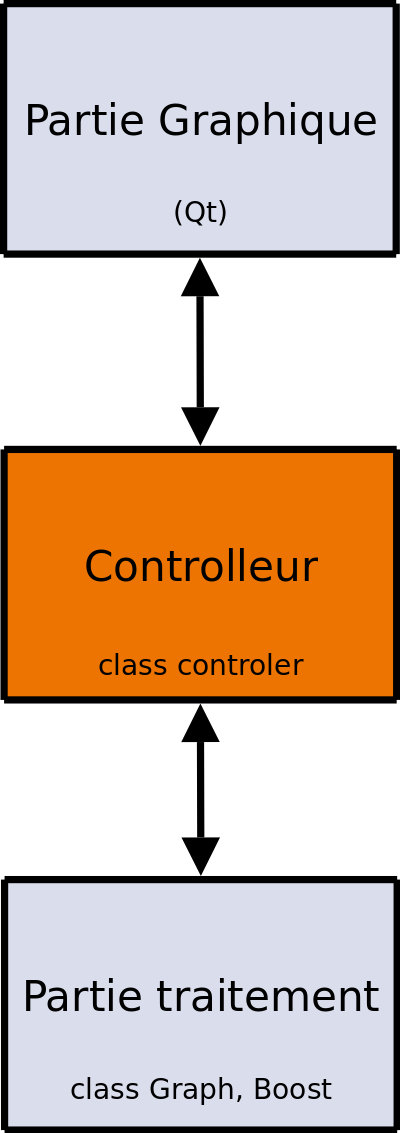
\includegraphics[height=0.3\textheight]{./schema/mvcScheme.png}
\caption{Schéma superficiel du Modèle Vue Controlleur}
\label{mvc}
\end{center}
\end{figure}

\subsubsection{La base du développement : l'objet Graph}

Dès le départ, nous savions que nous allions manipuler un graphe. Nous avons, avec l'aide de notre tuteur, créé un objet Graph à partir des classes exisantes dans \textit{Boost} nous permettant de manipuler ce graphe. En fait, cette objet est un liste d'adjacence de \textit{Boost} que nous avons spécialisé en fonction de nos besoins.

Le contenu du graphe est identifié par des descripteurs, l'un pour les sommets, \verb|vertex_descriptor| et l'autre pour les arêtes, \verb|edge_descriptor|. Bien que ces descripteurs soient des simples entiers, il ne nous était pas possible d'utiliser les numéros des AS. \textit{Boost} génère donc un entier auto-incrémenté utilisé comme identifiant vis à vis d'un objet AS contenant notamment son véritable numéro. Cette objet est stocké par le Graph.

Notre utilisation de l'objet graph ressemble à celui que l'on ferait d'une base de données. En considérant l'objet Graph comme tel, nous possèderions une table de sommets, et une table d'arêtes. La clé primaire de chacune de ces tables serait le descripteur correspondant (\verb|edge_descriptor| et \verb|vertex_descriptor|). Et nos entités seraient en faites des objets AS et ASLink (figure \ref{bdd}).

Ces objets possèdent un certain nombre d'attributs nécessaires au bon fonctionnement de boost en plus de ceux qui nous intéressent : le type et le numéro de l'AS. Pour récupérer le type de l'un de ces objets il suffit de faire \verb|graph[descriptor].type|.


\begin{figure}[H]
\begin{center}
        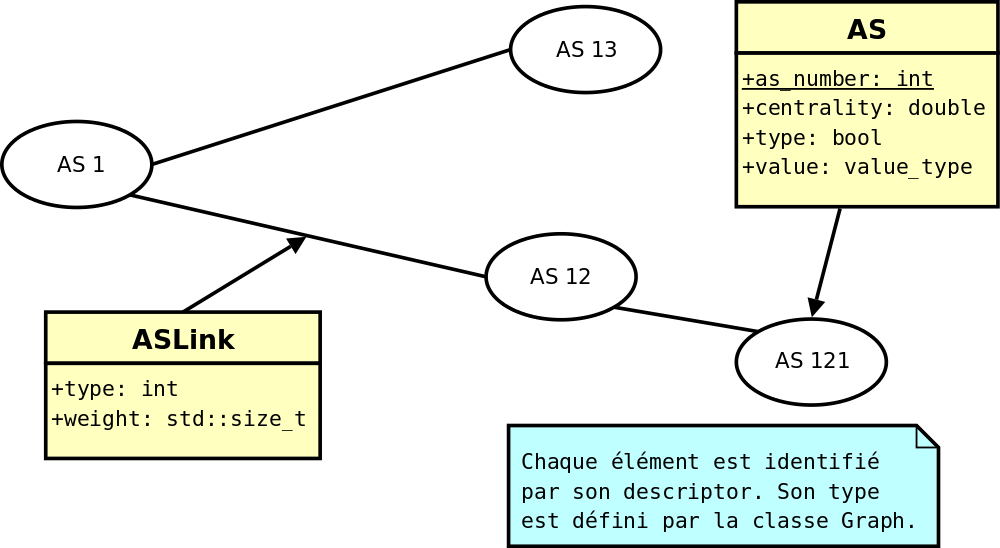
\includegraphics[width=0.8\textwidth]{./schema/bdd.png}
\caption{Représentation des types d'objet du graphe}
\label{bdd}
\end{center}
\end{figure}

\subsubsection{Représentation idéale}
Idéalement la représentation que nous souhaitions obtenir de vait tendre vers celle de la figure \ref{ideal}. 
\begin{figure}[H]
\begin{center}
        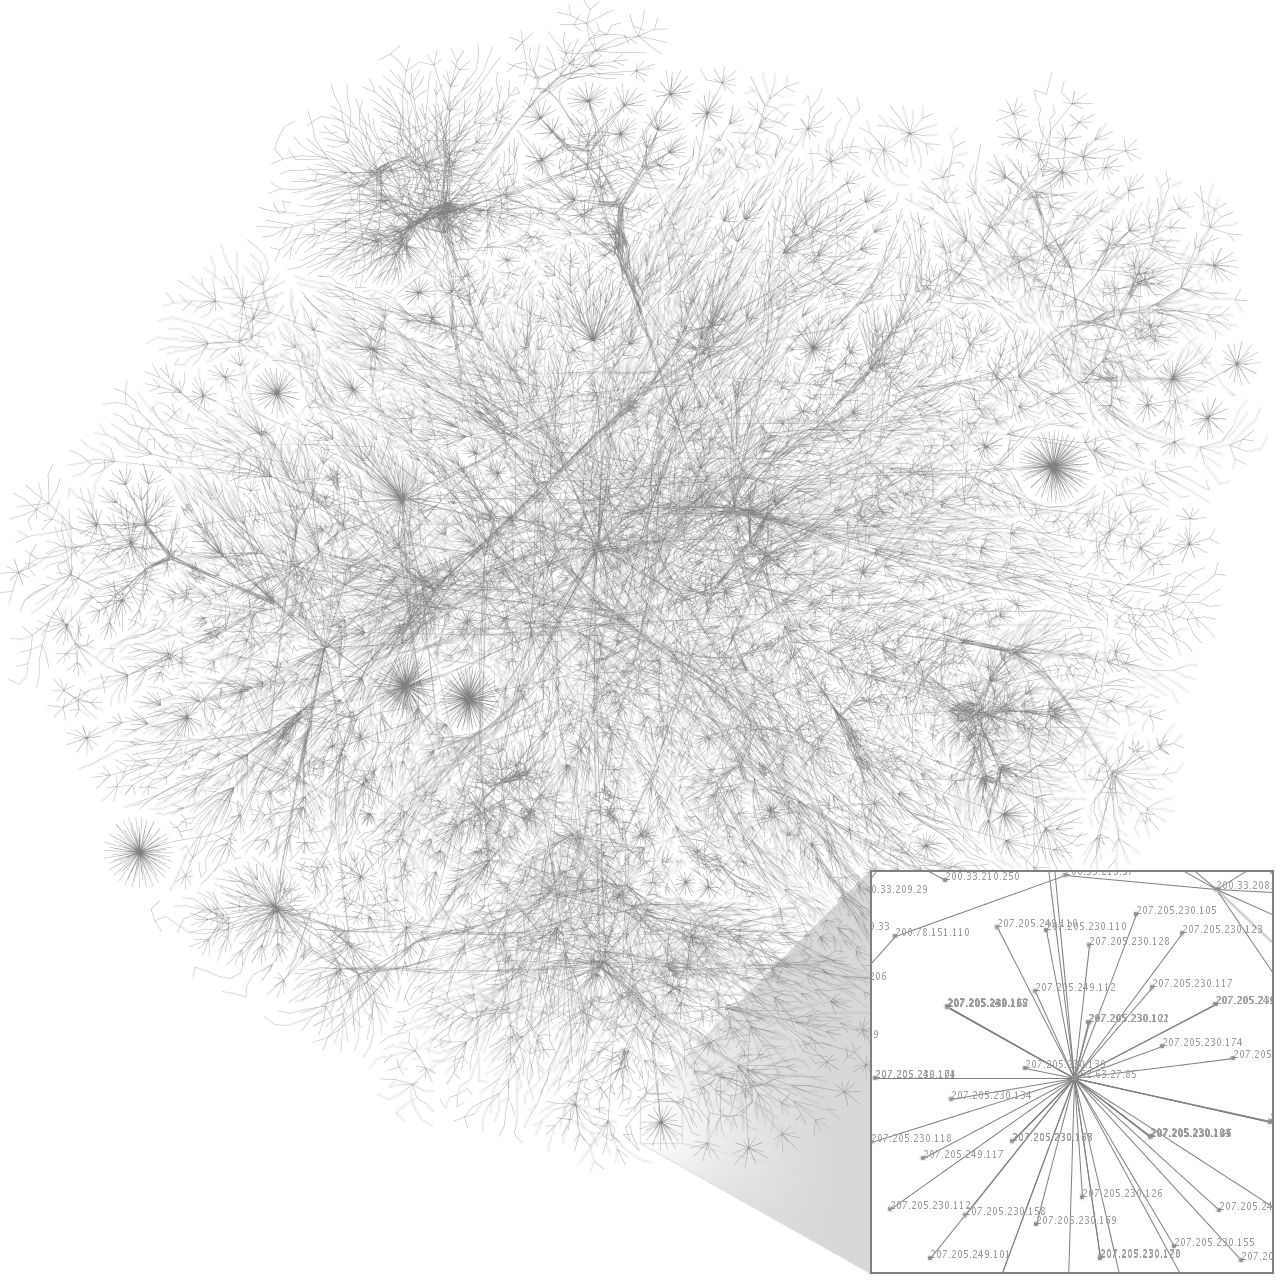
\includegraphics[width=0.8\textwidth]{./schema/Internet_map_1024_transparent.png}
\caption{Représenation idéale d'internet avec le programme}
\label{ideal}
\end{center}
\end{figure}


\pagebreak
\section{Solution r\'ealis\'ee}

\begin{frame}
 	\frametitle{Solution r\'ealis\'ee}
        \tableofcontents[currentsection,hideothersubsections]
\end{frame}

\subsection{Fonctionnalit\'es impl\'ement\'ees}
\frame
{
\frametitle{Fonctionnalit\'es impl\'ement\'ees}
\only<1>{
Fonctionnalit\'es du programme final :
\begin{itemize}
 \item R\'ecup\'eration d'informations sur un AS,
 \item Calcul du nombre de cliques maximum dans le graphe gr\^ace \`a l'algorithme de Bron and Kerbosch,
 \item Chargement d'un fichier de triplets pour \'eliminer les stubs du graphe,
 \item Zoomer sur le proche voisinage d'un AS,
 \item Revenir au graphe de base,
 \item Calculer la centralit\'e de Freeman des sommets,
 \item Filtrer les sommets selon leur centralit\'e,
 \item Filtrer les sommets selon leur num\'ero d'AS.
\end{itemize}
}
\only<2>{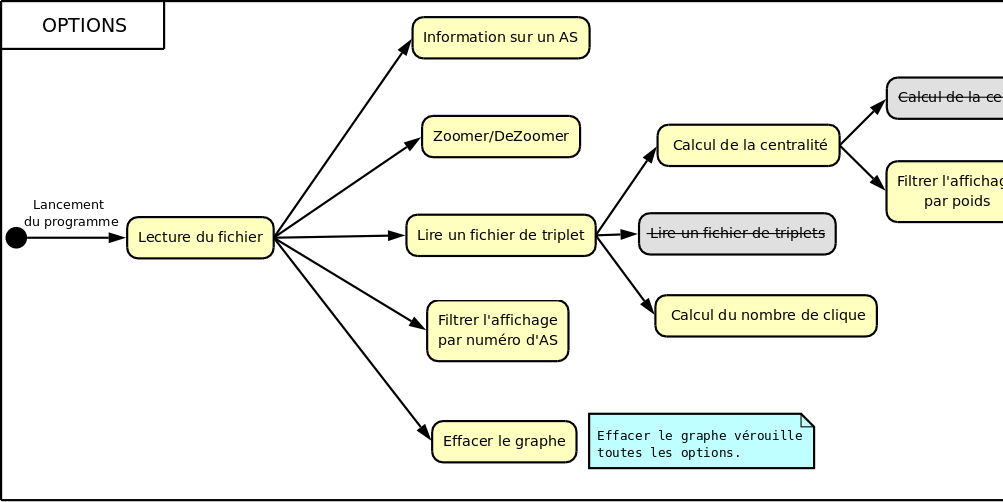
\includegraphics[width=\textwidth]{./seqMenu.png}}
}

\subsection{Rendu final}
\frame
{
\frametitle{Rendu final}
\only<1>
{
   \begin{center}
   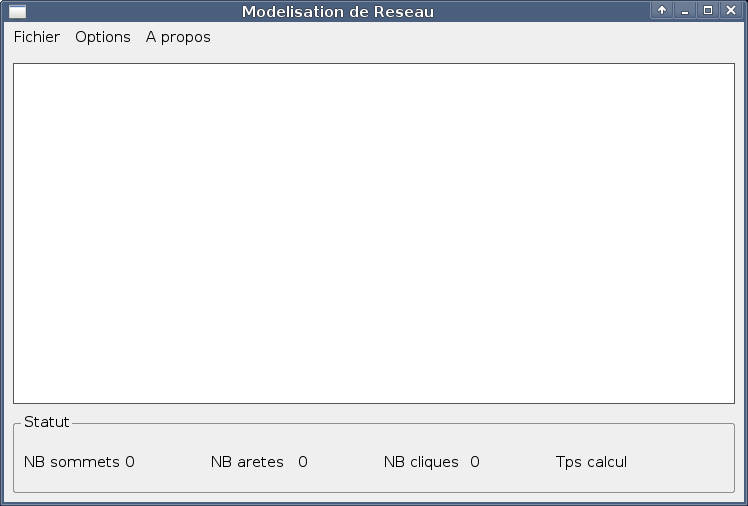
\includegraphics[width=0.9\textwidth]{ecran_programme.png}\\
   Ecran principal du programme
   \end{center}
}
\only<2>
{
   \begin{center}
   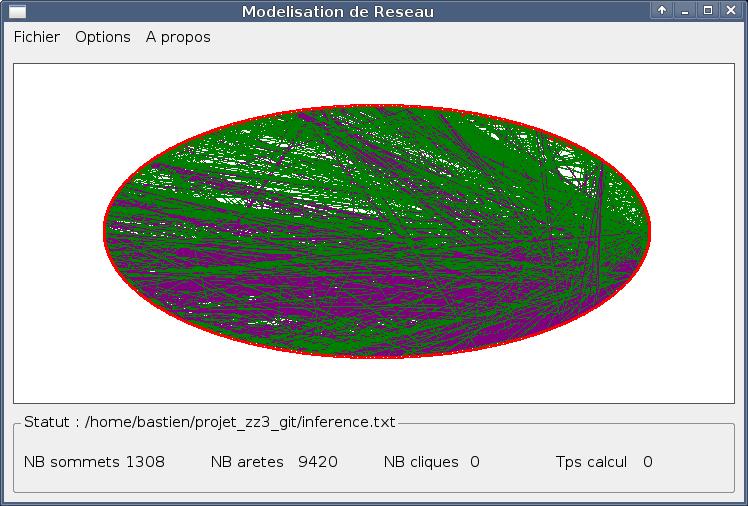
\includegraphics[width=0.9\textwidth]{ecran_graphe.png}\\
   Graphe charg\'e
   \end{center}
}
\only<3>
{
   \begin{center}
   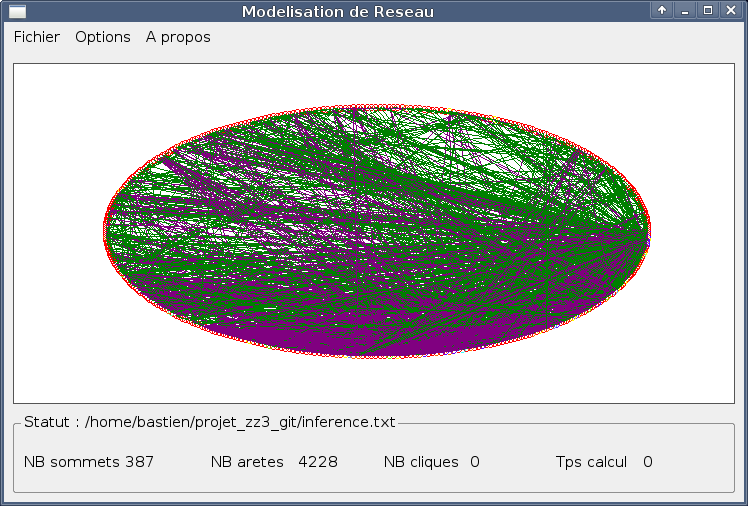
\includegraphics[width=0.9\textwidth]{ecran_graphe_nostubs.png}\\
   Stubs \'elimin\'es
   \end{center}
}
\only<4>
{
   \begin{center}
   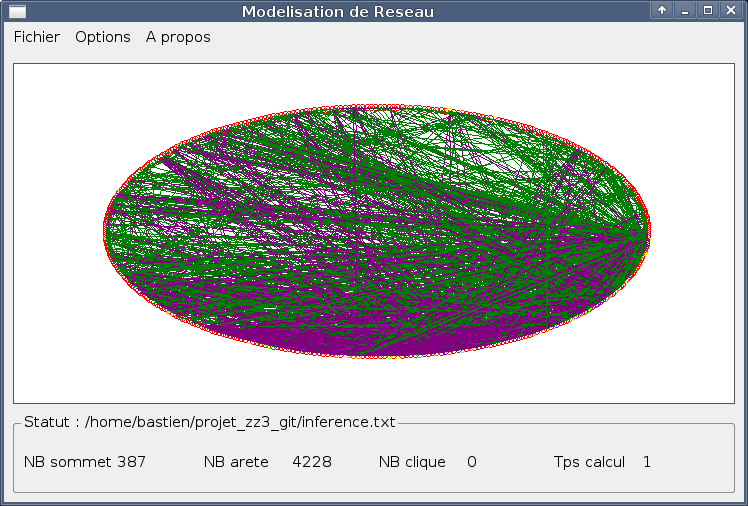
\includegraphics[width=0.9\textwidth]{ecran_graphe_centrality.png}\\
   Centralit\'e calcul\'ee
   \end{center}
}
\only<5>
{
   \begin{center}
   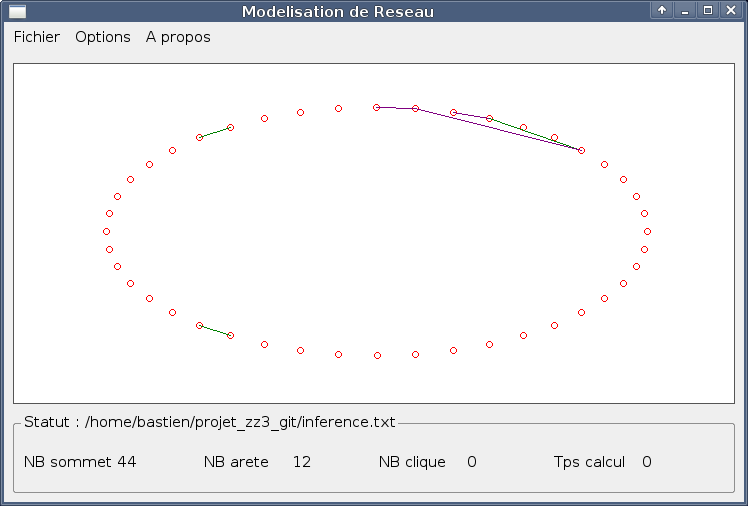
\includegraphics[width=0.9\textwidth]{ecran_graphe_filtre.png}\\
   Filtrage par num\'ero d'AS
   \end{center}
}
\only<6>
{
   \begin{center}
   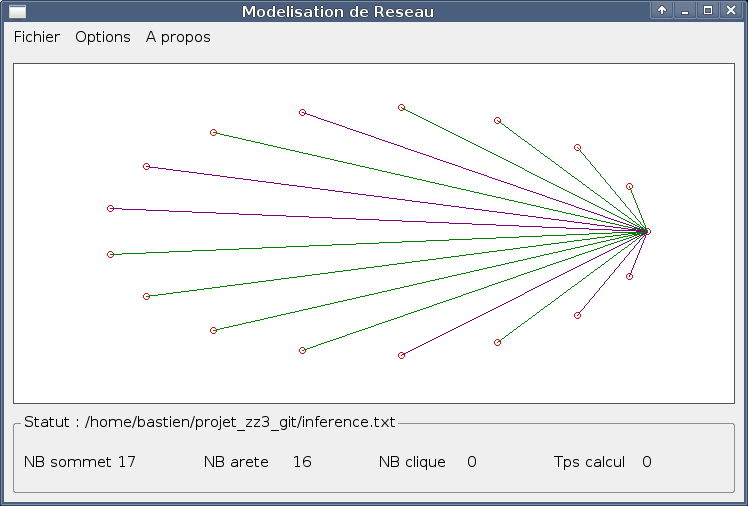
\includegraphics[width=0.9\textwidth]{ecran_graphe_zoom.png}\\
   Zoom sur un AS
   \end{center}
}
}
%\pagebreak
%\fancyhead[R]{Conclusion}
	%\section*{Conclusion}

\frame
{
\frametitle{Conclusion}
\framesubtitle{Analyse, représentation et évolutivité}

 \begin{itemize}
 \item Une première idée de représentation
 \item Identification des caractéristiques de l'Internet
 \item Filtrage de l'affichage
 \item Modèle-Vue-Contrôleur
 \end{itemize}

 

}

\frame
{
\frametitle{Conclusion}
\framesubtitle{Base à l'implémentation de nouvelles fonctionnalités}

 \begin{itemize} 
 \item Algorithmes d'analyse
% \begin{itemize}
\begin{description}
 \item[] \small{\emph{Connexité du graphe}}
 \end{description}
% \item 
% \end{itemize}
 \item Algorithmes d'affichage
% \paragraph{}
\begin{description}
 \item[] \small {\emph{ Kamada Kawai Spring Layout}}
 \end{description}

% 
 \item Améliorations de l'affichage 
% \paragraph{}

\begin{description}
 \item[] \small{\emph{Affichage des numéros d'AS quand on zoom}}
 \end{description}
% 
 \end{itemize}
\vfill

\begin{verse}
 `` \textit{Représenter la topologie de l'Internet est un challenge scientifique. }''
\end{verse} 

}
%\pagebreak
%\fancyhead[R]{Bibliographie}
%\input{./biblio.tex}
	% et enfin le contenu	
	\fancyhead{}
	\fancyhead[R]{\rightmark}
	\pagenumbering{arabic}
	
	
\pagebreak

\vfill
	
\vfill
\pagebreak
	
%	\input{biblio.tex}
\end{document}

%\usepackage{geometry}
%\geometry{hmargin=1.5cm, vmargin=1.5cm}

%\geometry{scale=0.8, nohead}

%\newenvironment{changemargin}[0]{\begin{list}{}{
	%\setmarginsrb{1.5cm}{1.5cm}{1.5cm}{1.5cm}{2.84cm}{2cm}{2.84cm}{2cm}
%}\item }{\end{list}}
%Idée de développement partir de Blancarde, pour arrivée à l'IVPico, ou l'inverse à voir. A l'oral ce serait certainement mieux, tellement Blancarde version installation est simple par rapport à l'autre.